\chapter{TIES AND THE ROBUSTNESS OF THE LEXIMIN ALGORITHM} \label{ch:robustness}% Must have a blank line after every section label

\epigraph{If in physics there's something you don't understand, you can always hide behind the uncharted depths of nature. You can always blame God. You didn't make it so complex yourself. But if your program doesn't work, there is no one to hide behind. You cannot hide behind an obstinate nature. If it doesn't work, you've messed up.}{Edsger Dijkstra}

\noindent In this chapter, I establish two beneficial properties of the leximin method. First, I show that the leximin method improves on popular methods because it recognizes \emph{ties} when there is no inherent ordering of cuts. Other methods break ties arbitrarily. The leximin method can perform multiway partitions instead of only splitting into two parts at each level of the dendrogram. The leximin method does not recognize ties which aren't there, when there is a community structure to the data. The second beneficial property is that the leximin method is robust to perturbations in the structure of the graph, in a way that competing algorithms are not.





\section{Introduction}

Any definition of hierarchical communities must align to our intuitive notions, or it is useless. One facet of this intuition is the ability to recognize \emph{ties}: multiple sub-communities that separate from one another at the same level in the hierarchy (e.g.\ \autoref{fig:dendrogram_3_tie_inverted}). This avoids imposing arbitrary community structure. Graphs like the complete graph $K_n$, which is fully connected, have no clear division into communities; we contend that a community detection technique ought to recognize that.

In addition, we would expect that small changes to the graph structure would smoothly affect the hierarchical structure, rather than causing discontinuous jolts or catastrophic alterations. More succinctly, our method should be \emph{robust} to changes in graph topology.

Understanding both ties and the robustness of the leximin method requires an understanding of the corresponding dual problem to the linear program which guides the leximin method. An overview of linear programming is given in \autoref{app:LP}. Importantly, from the corresponding dual to the HMCFP program, we can determine for each edge a range of values that its capacity can assume without changing the set of critical edges.

We can imagine the capacities of a particular graph as a point in $m$-dimensional space, where $m$ is the number of edges. The stability ranges define a convex polyhedron in that space, within which the set of critical edges is identical. For non-trivial problems (i.e.\ more than one edge), each polyhedron will be adjacent to other convex polyhedra. The set of all points within and along boundaries of all these polyhedra in $\mathbb{R}_{\geq 0}^m$ is equal to $\mathbb{R}_{\geq 0}^m$.

When the capacity of an edge moves beyond its stability range, we see a phase transition of sorts: the set of critical edges changes, leading to a different dendrogram. At the boundary between these regions, in analogy to phase transitions in physical matter, there is a coexistence of the states on either side of the boundary. The stability range of capacities at this transition is tight: only the current value can produce the observed behavior. This in-between state is one way to achieve a multipartite partition at a single level. (The other way is gridlock, discussed in \autoref{ch:random}.) This motivates our definition of a tie:

\begin{definition}{Tie} \label{def:tie}

A coincident set of cuts at one throughput level~$z$ that partitions the graph into more than two parts. No critical edge's capacity can be altered without \say{breaking} the tie: changing the set of critical edges.
\end{definition}

The remainder of the chapter illustrates the stability behavior of the leximin method on toy networks and a real-world example. I show that the leximin method exhibits smooth transition behavior, unlike the related MCF cut algorithm. On the examples, I show that popular algorithms are deficient in capturing intuitive notions of what a hierarchical community structure should be. Further, I compare the five hierarchical algorithms identified in \autoref{ch:literature} (Girvan--Newman edge betweenness, Fastgreedy, Walktrap, Leading Eigenvector, and MCF Cut) against the leximin method on the $K_3$ graph and the NFL matchup network from Mann et al.~\cite{mann2008sparsest}.




\section{Stability}

\begin{figure}
\centering
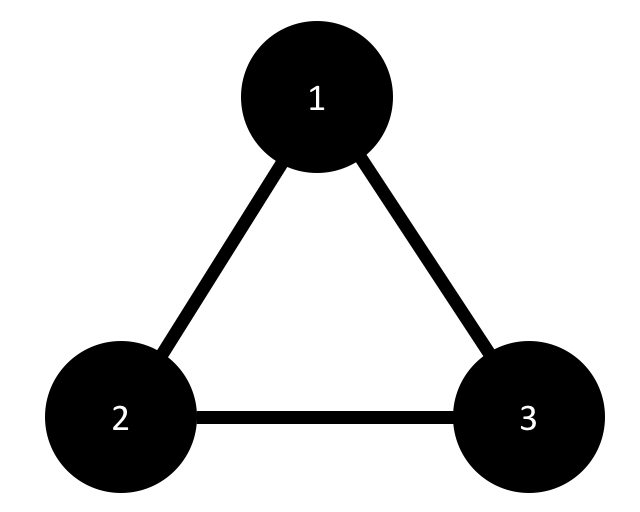
\includegraphics[width=0.6\textwidth]{fig/K3}
\caption{The complete graph on three vertices, $K_3$}
\label{fig:K3}
\end{figure}

\begin{figure}
\centering
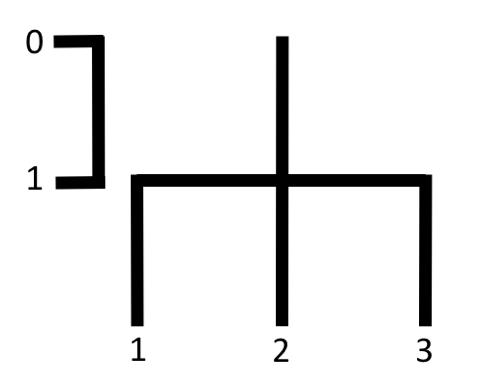
\includegraphics[width=0.6\textwidth]{fig/dendrogram_3_tie_inverted}
\caption{The dendrogram of ideal clustering of $K_3$ is a tie between all elements. This is recoverable by the MCF cut and leximin methods.}
\label{fig:dendrogram_3_tie_inverted}
\end{figure}


The complete graph on three vertices,~$K_3$, is shown in \autoref{fig:K3}. This graph shows the smooth transition between states. When we assign unit capacities to every edge, we see a fragmentation behavior. All edges saturate simultaneously at throughput $z=1$. This is a tie, according to Definition \autoref{def:tie}, and is shown in \autoref{fig:dendrogram_3_tie_inverted}. To show that this is a phase transition, we examine the behavior when any edge capacity is perturbed.

Without loss of generality, we can label its edges $i$, $j$, and $k$ and decide that their capacities obey $c_i \leq c_j \leq c_k$. Our method identifies two edges $i$ and $j$ as critical, then $i$ and $k$.  The stability ranges for $i$ and $j$ in the first cut are $[0, c_j]$ and $[c_j, c_j]$\footnote{There is some debate about whether an interval must contain more than one point. For our purposes, it is helpful to ignore this restriction.}, respectively, and the ranges for $j$ and $k$ in the second cut are $[c_j, c_j]$ and $[0, \infty)$. 

First, we examine the first cut. The capacity of $i$ can assume any value less than or equal to $c_j$ because there is no more constraining edge. No matter what, it will be saturated in the first cut. (An edge case: when the capacity is zero, this is equivalent to the edge not existing, in which case the remainder of the hierarchy remains the same.) The capacity of $j$ is bound to the value $c_j$ to maintain our ordering principle: otherwise, $k$ would saturate before it. 

In the second cut, $c_k$ is the only unsaturated edge, so it can take on any value \emph{for that subproblem}. Still, the range of values is constrained from below by $c_j$: if $c_k$ were less than $c_j$, we would again violate our ordering principle. 

There are $3! = 6$ possible orderings of the three edge weights. Each ordering defines a convex polyhedron bounded by two half planes in $\mathbb{R}_{\geq 0}^3$, coming from the inequalities that define the ordering. In any one of these cases, the dendrogram is the same for all points in the range. But we also know that the number of dendrograms with only binary partitions~\cite{erdos1975refining}:
\begin{equation}
n! (n-1)! / 2^{n-1}.
\end{equation}
This gives only 3 non-tie states. This is because there is no order to the lowest-level children. When one edge is assigned the label $k$, it doesn't matter which of the other two is $i$ and which is $j$, because they produce the same dendrogram.

When $c_i = c_j = c_k = c^*$, the first and second cuts occur at the same level of throughput, namely $z=c*$. The second cut is a \emph{degenerate cut}~\cite{danna2012practical}, and we see a tie. Any time there is a tie, there must be one or more degenerate cuts~\cite{vilas2015divisive}.

Further study is required to investigate the spatial division for non-symmetric graphs.



\section{Linearity}

\begin{figure}
\centering
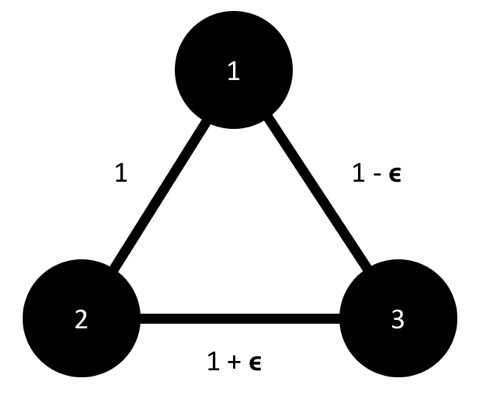
\includegraphics[width=0.6\textwidth]{fig/K3_perturbed}
\caption{$K_3$ with weights of two edges perturbed by $\epsilon$}
\label{fig:K3_perturbed}
\end{figure}

\begin{figure}
\centering
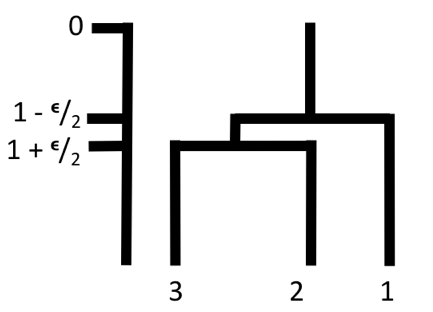
\includegraphics[width=0.6\textwidth]{fig/dendrogram_3_perturbed}
\caption{The dendrogram induced by perturbing the capacities of edges $\{1, 3\}$ and $\{2, 3\}$ by $-\epsilon$ and $+\epsilon$, respectively, shows robustness.}
\label{fig:dendrogram_3_perturbed}
\end{figure}

The $K_3$ graph gives a chance to show the linearity of the solutions across levels of the hierarchy. When the capacity of edge $i$ is decreased by $\epsilon$, the throughput at level 1 also decreases by $\frac{\epsilon}{2}$---that is, $\Delta z_1 = \Delta c_i / 2$. And when the capacity of $k$ is increased by $\epsilon$ as in \autoref{fig:K3_perturbed}, the throughput at level 2 rises by $\epsilon$ as in \autoref{fig:dendrogram_3_perturbed}. In other words, $z_2 = z_1 + \Delta c_k$. Because the LP for the second cut fixes the flows from level 1, it continues maximizing throughput from the same point. This preserves the linear relationship between \emph{shadow prices}\footnote{Shadow prices are explained in \autoref{app:LP}. For greater depth, see, e.g., Chvatal~\cite{chvatal1983linear}.} (changes in edge capacity) and changes in the objective function (i.e.\ throughput). The relationship holds for neighboring levels in the hierarchy.

Additionally, Matula has shown that when a dissimilarity value is used for cophenetic distance (i.e. dendrogram height) instead of throughput level, the leximin method exhibits smooth, linear response to perturbations, unlike the related MCF cut algorithm~\cite{matula1985divisive}.



\section{Ties: $K_3$}

The $K_3$ graph is sufficient to show a deficiency in the Girvan--Newman edge betweenness algorithm, Walktrap, and Fastgreedy: three hierarchical algorithms from the group considered in \autoref{ch:comparison}. Each fails to recognize \emph{ties} in height. The related paw graph additionally shows a deficiency in the fourth and fifth methods: Leading Eigenvector and MCF Cut.



\subsection{Intended Behavior}

The triangle should be split into three parts at the same level, because there is no difference between them, so one cannot impart an ordering. The dendrogram is represented by \autoref{fig:dendrogram_3_tie_inverted}.



\subsection{Observed Behavior}

The Girvan--Newman edge betweenness method imposes an arbitrary ordering\footnote{Any time an arbitrary ordering emerges, we note it. In terms of the methods' definitions, these choices are non-deterministic. The arbitrary selection presented here is always the same as was made by the \say{igraph} package implementation of each method.}: first separates node 1 from nodes 2 and 3, then separates those two. This is shown in \autoref{fig:dendrogram_3_no_tie_2}. Walktrap produces the same arbitrary ordering. Fastgreedy operates bottom-up to produce a different hierarchical clustering: it arbitrarily joins nodes 1 and 2 first, then joins node 3. The dendrogram for Fastgreedy is \autoref{fig:dendrogram_3_no_tie}. Leading Eigenvector produces a single split, seemingly recognizing the tie, as shown in \autoref{fig:dendrogram_3_tie}; in fact, it simply does not recognize any structure. This is because the leading eigenvector method is only capable of bifurcation, not splitting into an arbitrary number of components. The MCF cut and leximin techniques recognize the tie, reflecting the ideal behavior, as shown in \autoref{fig:dendrogram_3_tie_inverted}.

\begin{figure}
\centering
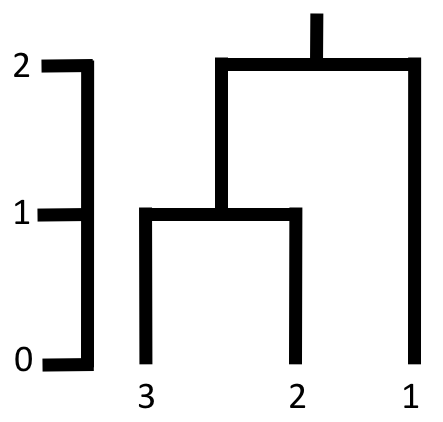
\includegraphics[width=0.6\textwidth]{fig/dendrogram_3_no_tie_2}
\caption{The dendrogram reflecting the arbitrary ordering induced by both edge betweenness (i.e. Girvan--Newman) and Walktrap on $K_3$}
\label{fig:dendrogram_3_no_tie_2}
\end{figure}

\begin{figure}
\centering
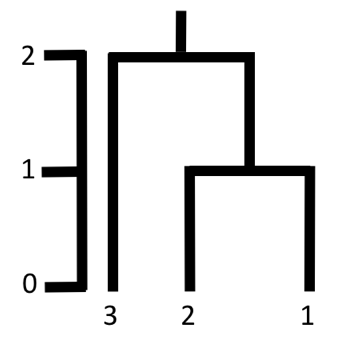
\includegraphics[width=0.6\textwidth]{fig/dendrogram_3_no_tie}
\caption{The dendrogram reflecting the arbitrary ordering induced by Fastgreedy on $K_3$}
\label{fig:dendrogram_3_no_tie}
\end{figure}

\begin{figure}
\centering
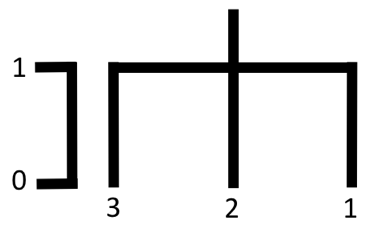
\includegraphics[width=0.6\textwidth]{fig/dendrogram_3_tie}
\caption{The dendrogram of clusterings recovered by leading eigenvector matches that of the leximin method, recognizing that there is no community structure. The sole difference is in the dendrogram height.}
\label{fig:dendrogram_3_tie}
\end{figure}



\subsection{Analysis}

The GN algorithm repeatedly removes the edge with highest edge betweenness centrality. In $K_3$, all edges are tied for betweenness centrality. GN will arbitrarily remove one edge, then another, then the last, splitting the network into two communities before it splits again into three at the next level in the hierarchy. The only monotonic metric that could be used for dendrogram height is the number of removed edges, and removing a single edge in a component can result in no more than two components. (This happens when the edge is a \emph{bridge}~\cite{west2001introduction} between two parts.) Because a tripartite cut (or, for that matter, a ($k > 2$)-partite cut is not possible, the GN dendrogram fails to handle the three-way tie. GN will have this problem for any symmetric graph, whether provided as input or induced as a step during its iteration.

Fastgreedy behaves similarly, although it is agglomerative (bottom--up): it merges exactly two communities at each level in the hierarchy, with no conception of ties. Modularity maximization is its guiding rule, and modularity is not monotonic, so we cannot use it as our dendrogram height. Additionally, regardless of the graph, modularity is provably different when any two clusters are joined, because the number of edges within clusters changes. Therefore, the tie can never be ameliorated as it is in both MCF cut and leximin.

Both the MCF cut algorithm and the leximin algorithm correctly compute the tie, albeit in a roundabout way. First, they each arbitrarily separate one node from the others, just like the other methods. At this point, the throughput is~$z=1$, and flow is necessarily on the shortest path between each pair. Next, the algorithm identifies the remaining edge as a critical edge, finishing the sequence of cuts. Importantly, the throughput for this cut is still~1. When we use throughput as our metric for height in the dendrogram, we correctly render a tied three-way split, as shown in \autoref{fig:dendrogram_3_tie_inverted}.

The refusal of Leading Eigenvector to impose an arbitrary ordering should not be misunderstood as a strength. It can only perform bipartite divisions. In this case, Leading Eigenvector failed to recognize any structure at all, halting immediately. It does the same for more intricate graphs like the paw graph, \autoref{fig:paw3}. In general, the method has poor performance~\cite{costa2007characterization} recognizing ground truth clusters.




\section{Real-World Ties and Sensitivity: The NFL Network}

\begin{figure}
\centering
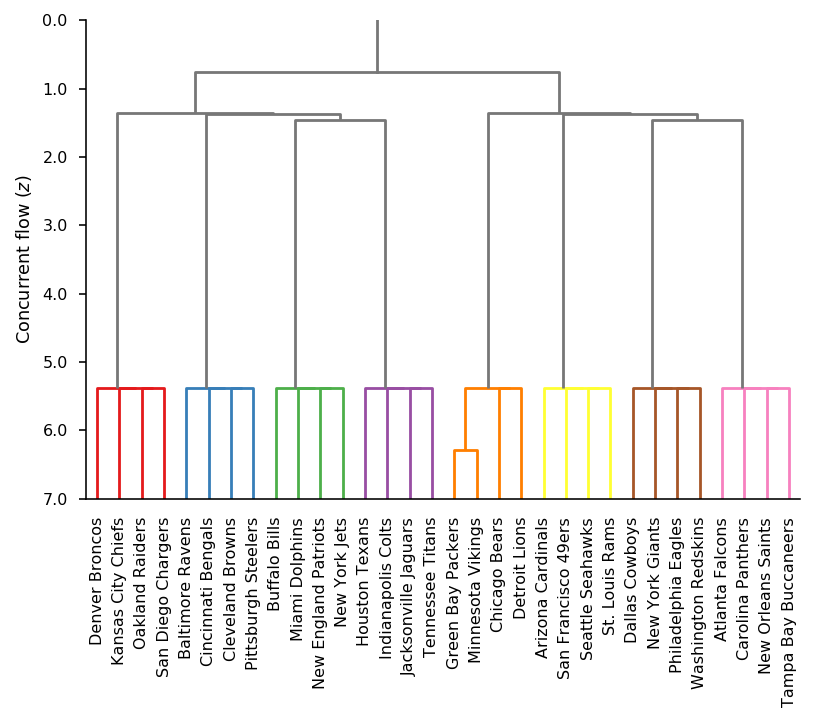
\includegraphics[width=0.8\textwidth]{fig/nfl}
\caption{Mann et al.'s network of NFL matchups, 2004--2006, clustered according to the leximin algorithm. The two conferences are split at the first level. Each colored group represents the North, South, East, or West division of a given conference.}
\label{fig:nfl}
\end{figure}

As a real-world example of when ties are important, consider the structure of National Football League (NFL) conferences and divisions. Mann et al.\ created a weighted network based on how often NFL teams played each other from 2004 to 2006~\cite{mann2008sparsest}. For a complete description, the reader is directed to Mann~\cite{mann2008extensions}.

The leximin method is able to recover the separation of the league into its two conferences. Additionally, it separates the eight divisions into their constituent teams. Using throughput as a measure of cophenetic distance gives a very tight grouping of the levels that separate the complete league from the divisions. Because the teams play each other without total regularity of frequency, it is unsurprising that the conferences don't splinter apart at the same level. Year-by-year differences in schedules have an impact. Consequently, this graph can be related to the perturbed triangle example: slight alterations in edge weights (capacities) would produce a uniform tie. Additionally, there exists parallel structure between the conferences. They are split at the same level as one another. This informs us that the structure of one conference has extremely similar structure to the other; its internal cohesion is not any stronger or weaker.

By their design, the other hierarchical methods under consideration perform bifurcations. They attempt to order the teams within divisions, when they are designed not to have any hierarchy. This indicates a deficiency in this use case.


\section{Discussion}

We have shown that the behavior of the leximin method is robust in the face of perturbations to graph structure. We have defined the specific constraints that will produce a tie. Finally, we have shown that no popular community detection method can identify ties in hierarchical structure. In the following section, we will examine the case of multipartite partitions which are not ties: a behavior of the leximin method called \emph{gridlock}.

%\section{Smoothness: The Paw Graph}
%
%The paw graph, introduced in \autoref{sec:differences}, demonstrates the deficiency in the MCF Cut algorithm. In this experiment, we assign capacities to each edge such that all edges are saturated simultaneously. Particularly, the capacity of $\{1, 2\}$ is $1/3$, the capacity of $\{1, 3\}$ and $\{2, 3\}$ is $2/3$, and the capacity of $\{3, 4\}$ is 1. The optimal assignment of flows to paths is shown in \autoref{fig:level1}. This is necessarily the same for both methods because each solves an equivalent LP: There are not yet any fixed flows in the leximin method.
%
%\begin{figure}
%\centering
%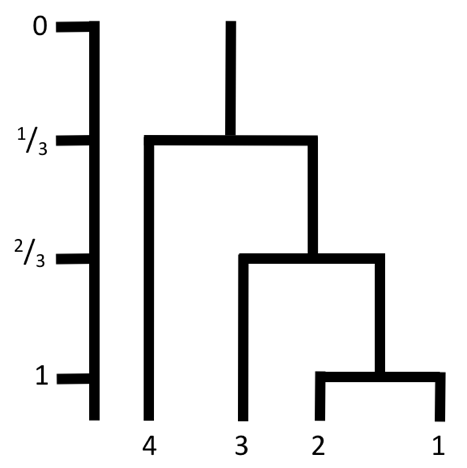
\includegraphics[width=0.6\textwidth]{fig/dendrogram_4_cascade}
%\caption{The dendrogram of clusterings recovered by the leximin method on the paw graph.}
%\label{fig:dendrogram_4_leximin}
%\end{figure}
%
%\begin{figure}
%\centering
%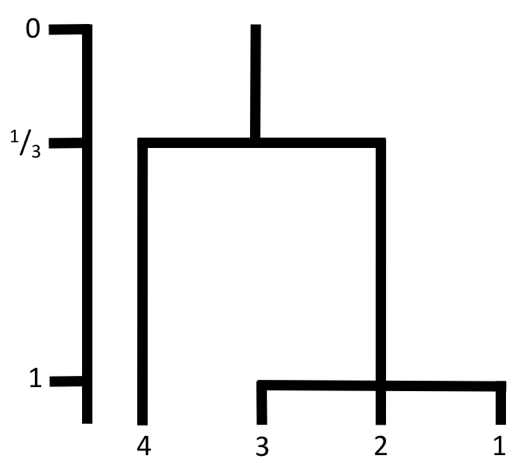
\includegraphics[width=0.6\textwidth]{fig/dendrogram_4_tie}
%\caption{The dendrogram of clusterings recovered by the MCF cut method on the paw graph.}
%\label{fig:dendrogram_4_MCF}
%\end{figure}
%
%The dendrograms produced by the leximin and MCF cut methods are shown in \autoref{fig:dendrogram_4_leximin} and \autoref{fig:dendrogram_4_MCF}. Of interest is the behavior when the graph is perturbed. When the leximin method is applied to a graph with diminished By contrast, the MCF cut algorithm produces a discontinuous series of cuts.
%
%\subsection{Maximin algorithm as a linear program} \label{sec:maximin LP}
%
%The salient difference between the maximin and MCF cut algorithms is that the MCF cut algorithm separates the graph and re-solves the MCFP on each component, while the maximin algorithm continues to solve the MCFP on the entire graph, with previously determined levels of flow fixed from variables into constants. We will denote as~$u_{ij}$ the sum of all flows from previous iterations across the edge~$\{i, j\}$. Also, in subsequent iterations, we remove from $D$ the set of saturated edges from previous iterations. Expanding on the definition provided by Matula~\cite{matula1985concurrent}, the \emph{hierarchical} MCFP's edge--path formulation is:
%\begin{align}
%    \max z(G, c, d)  & && \text{throughput} \nonumber\\
%    \mathrm{s.t.} \sum_{p \in P_{ij}} f_p &= zd_{ij} \forall \{i, j\} \in D && \text{fairness constraint} \nonumber\\
%    \sum_{\{p \in P:\{i,j\} \in E_p\}} f_p &\leq c_{ij} - u_{ij} \forall \{i, j\} \in E && \text{capacity constraint} \nonumber\\
%    f_p &\geq 0,  p \in P && \text{non-negativity of flow} \label{eq:mcfp-maximin}
%\end{align}
%

% \subsection{Interpretation}

% In the context of this problem, the shadow price represents the marginal increase in possible flow for a change in the edge's capacity~\cite{ahuja1993network}. Edges with a shadow price of zero have not become saturated; there is no additional benefit to increasing their capacity. Edges with nonzero shadow prices are \emph{critical edges}; depending on whether we use \autoref{alg:hmcfp} or \autoref{alg:hmcfp-cc}, we handle these differently and move to the next iteration.

% In Mann's formulation of the MCF cut algorithm, edges with nonzero shadow prices are critical edges which separate the graph into two or more components. One component is selected from the set of components; the MCFP is solved for this component to find new critical edges at a higher throughput level. In the consistent-components formulation, some edges may have a nonzero shadow price even though they were critical edges in a previous level of the hierarchy\todo{Show me with the Florentine families}. Increasing the capacity of these edges improves the current solution when all prior flows remain fixed; the impact on the entire hierarchy remains to be studied. To solve the next iteration of the HMCFP, the current flows become fixed, reducing the capacity of edges and eliminating demand between pairs across the cut or grid created by critical edges.

% An unusual observation which requires explanation is that when working down the hierarchy, an edge will be cut twice, only if that edge would contribute to the formation of a loop.

%paw graph
%edge betweenness: (4, ((3, 2), 1))
%walktrap: (4, (3, (1, 2)))
%leading eigenvector: tie
%fast greedy: ((1, 2), (3, 4)) <- 1, 2 at level 2 and 3, 4 at level 1; merge them at level 3
